\chapter{Application Controls}
\label{cs:ac}

Nota sull'esame: descrizione di un caso + poche domande

\begin{figure}[h!]
        \begin{center}
                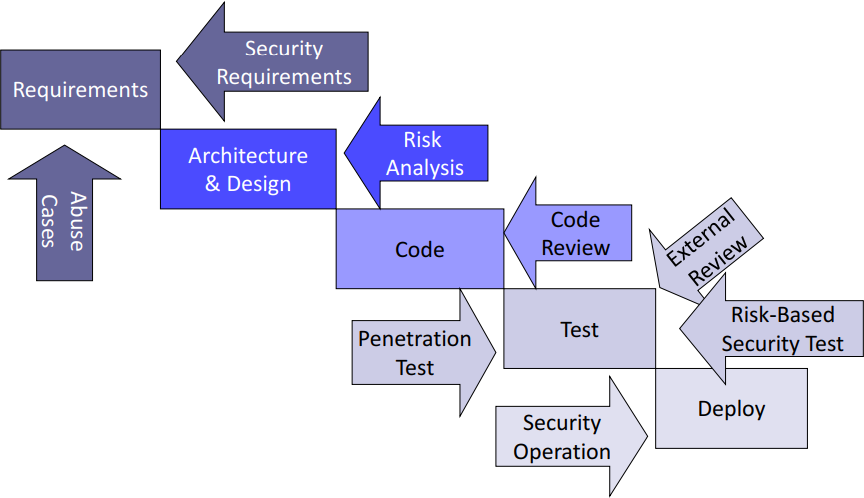
\includegraphics[width=\textwidth]{security_software_development}
        \end{center}
        \caption{La sicurezza nello sviluppo del software}
        \label{fig:security:software:development}
\end{figure}

Nell'immagine \ref{fig:security:software:development}:

\begin{enumerate*}[label=\alph*)]
	\item Abuse case (invece di use case) si riferisce ai  tipici casi in cui il 
	sistema può essere flesso in chiara violazione delle policy di 
	sicurezza. 
	\item La Code review consiste anche nell'analisi statica.
	\item Il Test sul software è inteso come penetration test, stress test, ecc.
\end{enumerate*}

\paragraph{Transaction Validation}
\begin{itemize}
	\item Sequence check: l'utilizzo di sequence number fanno sì che numeri
	out-of-sequence o numeri duplicati vengano rifiutati.
	\item Controllo dell'intervallo e limiti: i numeri sono sotto un numero
	massimo dato o in un intervallo specifico.
	\item Controlli di validità o lookup di una tabella:
	solo alcuni valori sono accettati (es. Sesso = M/F).
	\item Controlli di ragionevolezza: i valori inseriti sono ragionevoli.
	Per esempio per una pizzeria un'ordine di pizza d'asporto di 100 pizze
	va verificato.
	\item Controlli di esistenza: i campi richiesti da compilare
	sono completati correttamente.
	\item Key Verification: l'input è controllato due volte attraverso
	una seconda persona o tutte le cifre sono immesse due volte.
	\item Check Digit: una cifra potrebbe verificare la corretta
	immissione di altre cifre.
	\item Completeness check: viene immesso un input completo. Gli
	spazi o gli zero sono controllati per ogni lettera o cifra 
	richiesta \todo{Non chiaro il testo originale}.
	\item Duplicate Check: bisogna sempre controllare se una transizione
	con lo stesso ID esiste già. In caso affermativo va rifiutata.
	\item Consistency or Logical Relationship Check: i nuovi dati
	sono coerenti con altri dati a disposizione: per esempio
	la data di nascita di un dipendente deve essere avvenuta almeno
	16 anni fa.
\end{itemize}


\paragraph{Batch Processing} 
È un tipo di controllo dell'input.
Elaborazione sequenziale di blocchi di transazioni
dopo che sono state aggregate. 
L'input è autorizzato e raccolto in ``batch''. Vengono effettuati
dei controlli automatici su un batch e associati ad un batch file.
Viene effettuata la validazione della transazione. Le transazioni
rifiutate sono corrette e rimandate o trattate in altro modo.

Viene effettuato il processing (es. ordine pagamenti e salvataggio nel DB):
Il processing viene completato.
Infine segue il batch balancing attraverso 
una riconciliazione manuale o automatica dei controlli di batch.

\begin{figure}[h!]
        \begin{center}
                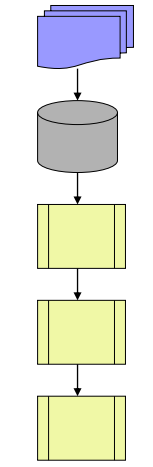
\includegraphics[scale=0.5]{batch_processing}
        \end{center}
        \caption{Batch processing}
        \label{fig:security:batch:processing}
\end{figure}

\paragraph{Transaction Authorization}
\begin{itemize}
	\item Manuale: Ottenimento della firma dal management 
	\item Automatico
\end{itemize}

Automatico

\paragraph{Error Handling Alternatives}
Il trattamento degli errori di input possono essere trattati
con le seguenti tecniche:
\begin{itemize}
\item Rigettare le transazioni con errori e continuare a processare 
il batch;
\item Rigettatre l'intero batch di transazioni, se contiene
degli errori.
\item Tieni il batch in sospeso fintanto che le transazioni 
non vengono fissate.
\item Accetta l'intero batch ma contrassegna le transazioni che
contengono degli errori per renderne più facile l'identificazione,
permettendo quindi futuri correzioni.
\end{itemize}


\subparagraph{Data Processing}

\begin{figure}[h!]
        \begin{center}
                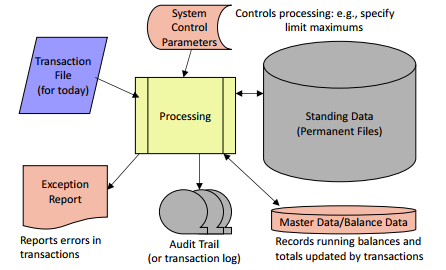
\includegraphics[width=\textwidth]{data_processing}
        \end{center}
        \caption{Data processing}
        \label{fig:data:processing}
\end{figure}

Il processing comprende controllo dei parametri di sistema (es. specificare
minimo e massimo), Standing data (file permanenti), report delle eccezioni
(errori nelle transazioni), log delle transazioni, file delle transazioni
(giornaliero).

\paragraph{Processing controls}
I processing controls sono usati per assicurare
l'accuratezza, la completezza e la validità dei dati durante
processing online o batch. Questi controlli sono messi in campo
per verificare che i dati vengano procesati solo tramite routine
autorizzate. Esistono due modi per eseguire i processing controls:

\begin{itemize}
\item \textbf{Eseguita transazione per transazione}
\begin{itemize}
\item Editing: il programma testa l'accuratezza, la completezza
e la validità dei dati.
\item Controlli sugli ammontare calcolati: i valori calclati
sono controllati per essere ragionevoli e non eccedere il massimo.
\item Controlli programmati: Software che rileva, logga e inizia
delle azioni correttive per gli errori.
\item Report delle eccezioni: gli errori delle transazioni vengono
riportati con il loro tipo di errore.
\end{itemize}

\item \textbf{Eseguita Batch per Batch}

\begin{itemize}
\item Batch Register:I batch totals sono salvati manualmente per essere
confrontati con i totals di sistema. 
\item Run-To-Run Totals: ogni passo del processing riporta i batch
controls calcolati
\item Reconciliation: un supervisore deve ricontrollare che \emph{tutti}
i dati sono stati salvati e processati correttamente.
\end{itemize}
\end{itemize}


\paragraph{Controllo sui file dati}
\begin{itemize}
\item
Prerecorded Input: Certain information fields are preprinted on a blank
input form to reduce input errors.
\item
Data File Security: solo l'accesso autorizzato è consentito.
\item
Version usage: è sempre usata la versione corretta di un file
\item
Transaction Logs: Un traccia per l'audit: salva la data e l'ora dell'input,
l'ID dell'utente, il terminal (su cui si è effettuata la transazione) e
l'input di transazioni.
\item
Before and After Image Reporting: Un file contenente dati è salvato
prima e dopo averlo processato. In questo modo è possibile tenere traccia
dell'impatto delle transizioni sui file.
\item 
Parity Checking: Quando un file è inviato, bisogna aggiungere dei codici
per il controllo, per asicurare che sia trasmeso senza errori (hash).
\end{itemize}

Controlli su \textbf{Batch Processing}:
\begin{itemize}
\item
Error reporting \& handing: tutti i report di errori sono stati riconciliati
e le autorizzazioni/correzioni sono state trasmesse in ordine temporale.
\item
One-for-One Checking: i documenti descrivono correttamente il processing
che è avvenuto.
\item
Source document retention: la gestione dei documenti è un'attività molto
onerosa perché richiede che ci sia una organizzazione in piedi.
\item
Internal \& External Labeling: c'è il backup, bisogna etichettarli in 
modo da trovare quello giusto.
\end{itemize}





\section{Esercizi}

Gli esercizi sono disponibili in \ref{esCs:ac}

\chapter{Application Audit}
\label{cs:aa}

I compiti dell'auditor includono:
\begin{itemize}
\item Identificare componenti signaficativi delle applicazioni e 
il flusso delle transazioni.
\item 
Identificare controlli appropriati e valutarne l'efficacia
\item 
Testare i controlli
\item Analizzare i risultati del singolo test per determinare se 
il controllo funziona come atteso: così si può giudicare se è inutile,
oneroso, o se è utile, ecc.
\end{itemize}

\todo{Insert image: Integrated testing facilities}
\begin{figure}[h!]
        \begin{center}
                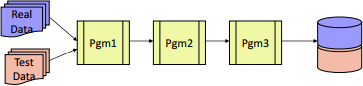
\includegraphics[width=\textwidth]{testing_facilities_integrated}
        \end{center}
        \caption{Strumenti di test integrati.}
        \label{fig:testing:facilities:integrated}
\end{figure}

\begin{figure}[h!]
        \begin{center}
                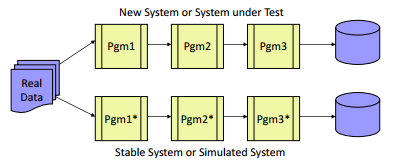
\includegraphics[width=\textwidth]{parallel_operation_simulation}
        \end{center}
        \caption{Operazioni o simulazioni parallele.}
        \label{fig:testing:facilities:parallel}
\end{figure}
si fa quando si vuole aggiornare i sistemi in produzione.

\todo{Insert image Embedded}
Embedded Audit Modules (EAM): il suo grande svantaggio È quello di rallentare il
sistema. Qualora vada tutto bene sono soldi spesi inutilmente.
Systems Control Audit Review File (SCARF):
Sample Audit Review File (SARF) scelta a campione non è più la scelta migliore.

\paragraph{Testing Application Techniques}
\todo{copia elenco}
Validate Systems $\Leftarrow$ Importanti Parallel Simulation e Parallel
Operation



\paragraph{Tecniche di Auditing Onine}
Audit Hooks:all'interno del codice ci sono delle condizioni particolari che se
sono soddisfatte triggerano delle operazioni di auditing, è meno pesante delle
EAM infatti viene attivato il controllo SOLO quando si raggiungono certi path
del CFG.
\todo{Copia  tabella}
\todo{Copia disegnino di Hook}

\section{Esercizi}

Gli esercizi sono disponibili in \ref{esCs:aa}

\part{Incident process process forensics}

Un incidente relativo alla sicurezza può capitare per molti problemi. Un
incidente è catalogato come tale quando c'è una violazione della \textit{policy}
di sicurezza. Un incidente può essere di due tipologie:
\begin{itemize}
\item Malizioso
\item Casuale (non malizioso)
\end{itemize}

\chapter{Incident Response vs Business Contiuity}
\label{IRBC}

Avere un piano di risposta agli incidenti fa parte della \textit{business
continuity plan}.

\section{Business Continuity Plan}

\subsection{Terminologia della \textit{recovery}}
\todo{Add refernce to old image --> RECOVERY TERMS}
Esiste una determinata tipologia di termini:
\begin{itemize}
\item Interruption Window
\item Service Delivery Objective
\item ?? \todo{Aggiungimi :(}
\end{itemize}

In particolare, esistono diversi ruoli che vedremo in dettaglio.

\paragraph*{IMT} L'IMT, che significa \textbf{Incident Management Team}, fa
parte della \textit{steering commitee} e sono membri dell'IRT. % va troppo
veloce




\paragraph*{IRT} L'IRT, che significa \textbf{Incident Response Team}, ed è il
team che gestisce l'incidente, ha una conoscenza tecnica dei sistemi e di
``hacking'' (è il classico informatico)

\paragraph*{Investigatore} Presenti in aziende grandi, è una persona di fiducia
che ha accesso a tutte le risorse aziendali e si occupa di cercare le cause
dell'incidente che a volte possono anche essere dolose.



\subsection{Incident Response Plan}

Questo piano si suddivide in diversi \textit{step}:
\begin{enumerate}
\item Preparazione
\item Identificazione
\item Contenimento
\item Analisi e eradicazione
\item Recupero
\item Imparare
\end{enumerate}

Vediamo brevemente il significato di ogni passo, che sarà analizzato in
profondità più avanti.

\paragraph*{Preparazione} Questa fase è la preparazione dell'incidente, ovvero è
una fase che è l'\textbf{analisi dello scenario}.

\paragraph*{Identificazione} Questo \textit{step} succede quando si viene
avvisati dell'anomalia e si comincia a cercare la causa del problema. Più e
ricco e sistema il complesso informativo più è difficile trovare la causa del
problema.

\paragraph*{Contenimento} In questa fase si cerca di ``limitare i danni'', con
l'obiettivo di mantenere l'operatività. Questo a volte consiste in sacrificare
elementi della produttività.

\paragraph*{Analisi e eradicazione} Si cerca di capire cos'è successo e perchè è
successo, e si cerca di risolvere la causa.

\paragraph*{Recupero} Si ritorna con i servizi di nuovo funzionanti, per
ritornare alla fase di preparazione

\paragraph*{Imparare} Questa parte è molto importante, in quanto imparare la
lezione permette di evitare futuri attacchi e di rendere il sistema più sicuro.
